% https://ayearofai.com/rohan-lenny-1-neural-networks-the-backpropagation-algorithm-explained-abf4609d4f9d#.22pxx8bi2
% https://ayearofai.com/rohan-4-the-vanishing-gradient-problem-ec68f76ffb9b#.lwknz63ef

\documentclass[ppt3]{ppt}

\usetikzlibrary{arrows,calc,decorations.markings,math,arrows.meta}
\usetikzlibrary{matrix,chains,positioning,decorations.pathreplacing,arrows}

\usepackage{lipsum}
\makeatletter
  \renewcommand\lips@dolipsum{%
    \ifnum\value{lips@count}<\lips@max\relax
      \addtocounter{lips@count}{1}%
      \csname lipsum@\romannumeral\c@lips@count\endcsname
      \lips@dolipsum
    \fi
  }
\makeatother

\newcommand{\titulo}{\insertsectionhead}
\newcommand{\subtitulo}{\insertsubsectionhead}
\newcommand{\subsubtitulo}{\insertsubsubsectionhead}

\institute[USACH]{Universidad de Santiago de Chile\\Facultad de Ingeniería\\Magíster en Ingeniería Informática}
\title{Algoritmos Genéticos y el problema del desvanecimiento del gradiente}
\subtitle{Informe III}
\author[Reyes F.]{Felipe Reyes González}
\date{\today}


\begin{document}

\thispagestyle{empty}
\begin{frame}{\titulo}{\subtitulo}
\maketitle
\end{frame}

\thispagestyle{empty}
\begin{frame}{\titulo}{\subtitulo}
	\tableofcontents
\end{frame}
\setcounter{framenumber}{0}

%\section{Introducción}
\begin{frame}{\titulo}{\subtitulo}
    \begin{itemize}
        \item Las redes neuronales no son más que muy buenos aproximadores de función.\bigskip

        \item Le das una red entrenada, un vector de entrada, realiza una serie de operaciones, y se produce un vector de salida.\bigskip

        \item Para entrenar a nuestra red para que estimar una función desconocida, le damos una colección de puntos de datos o {\bf conjunto de entrenamiento} que la red va a aprender y generalizar para hacer inferencias futuras.
    \end{itemize}
\end{frame}

\begin{frame}{\titulo}{\subtitulo}
    \begin{itemize}
        \item Las redes neuronales se estructuran como una serie de capas.\bigskip

        \item Cada capa está compuesta de una o más neuronas.\bigskip

        \item Cada neurona produce una salida, o se activa, basándose en las salidas de la capa anterior y un conjunto de pesos.
    \end{itemize}
    \begin{figure}[H]
        \centering
        \scalebox{0.6}{%!tikz editor 1.0
\documentclass{article}
\usepackage{tikz}
\usepackage[graphics, active, tightpage]{preview}
\PreviewEnvironment{tikzpicture}

%!tikz preamble begin

%!tikz preamble end


\begin{document}
%!tikz source begin
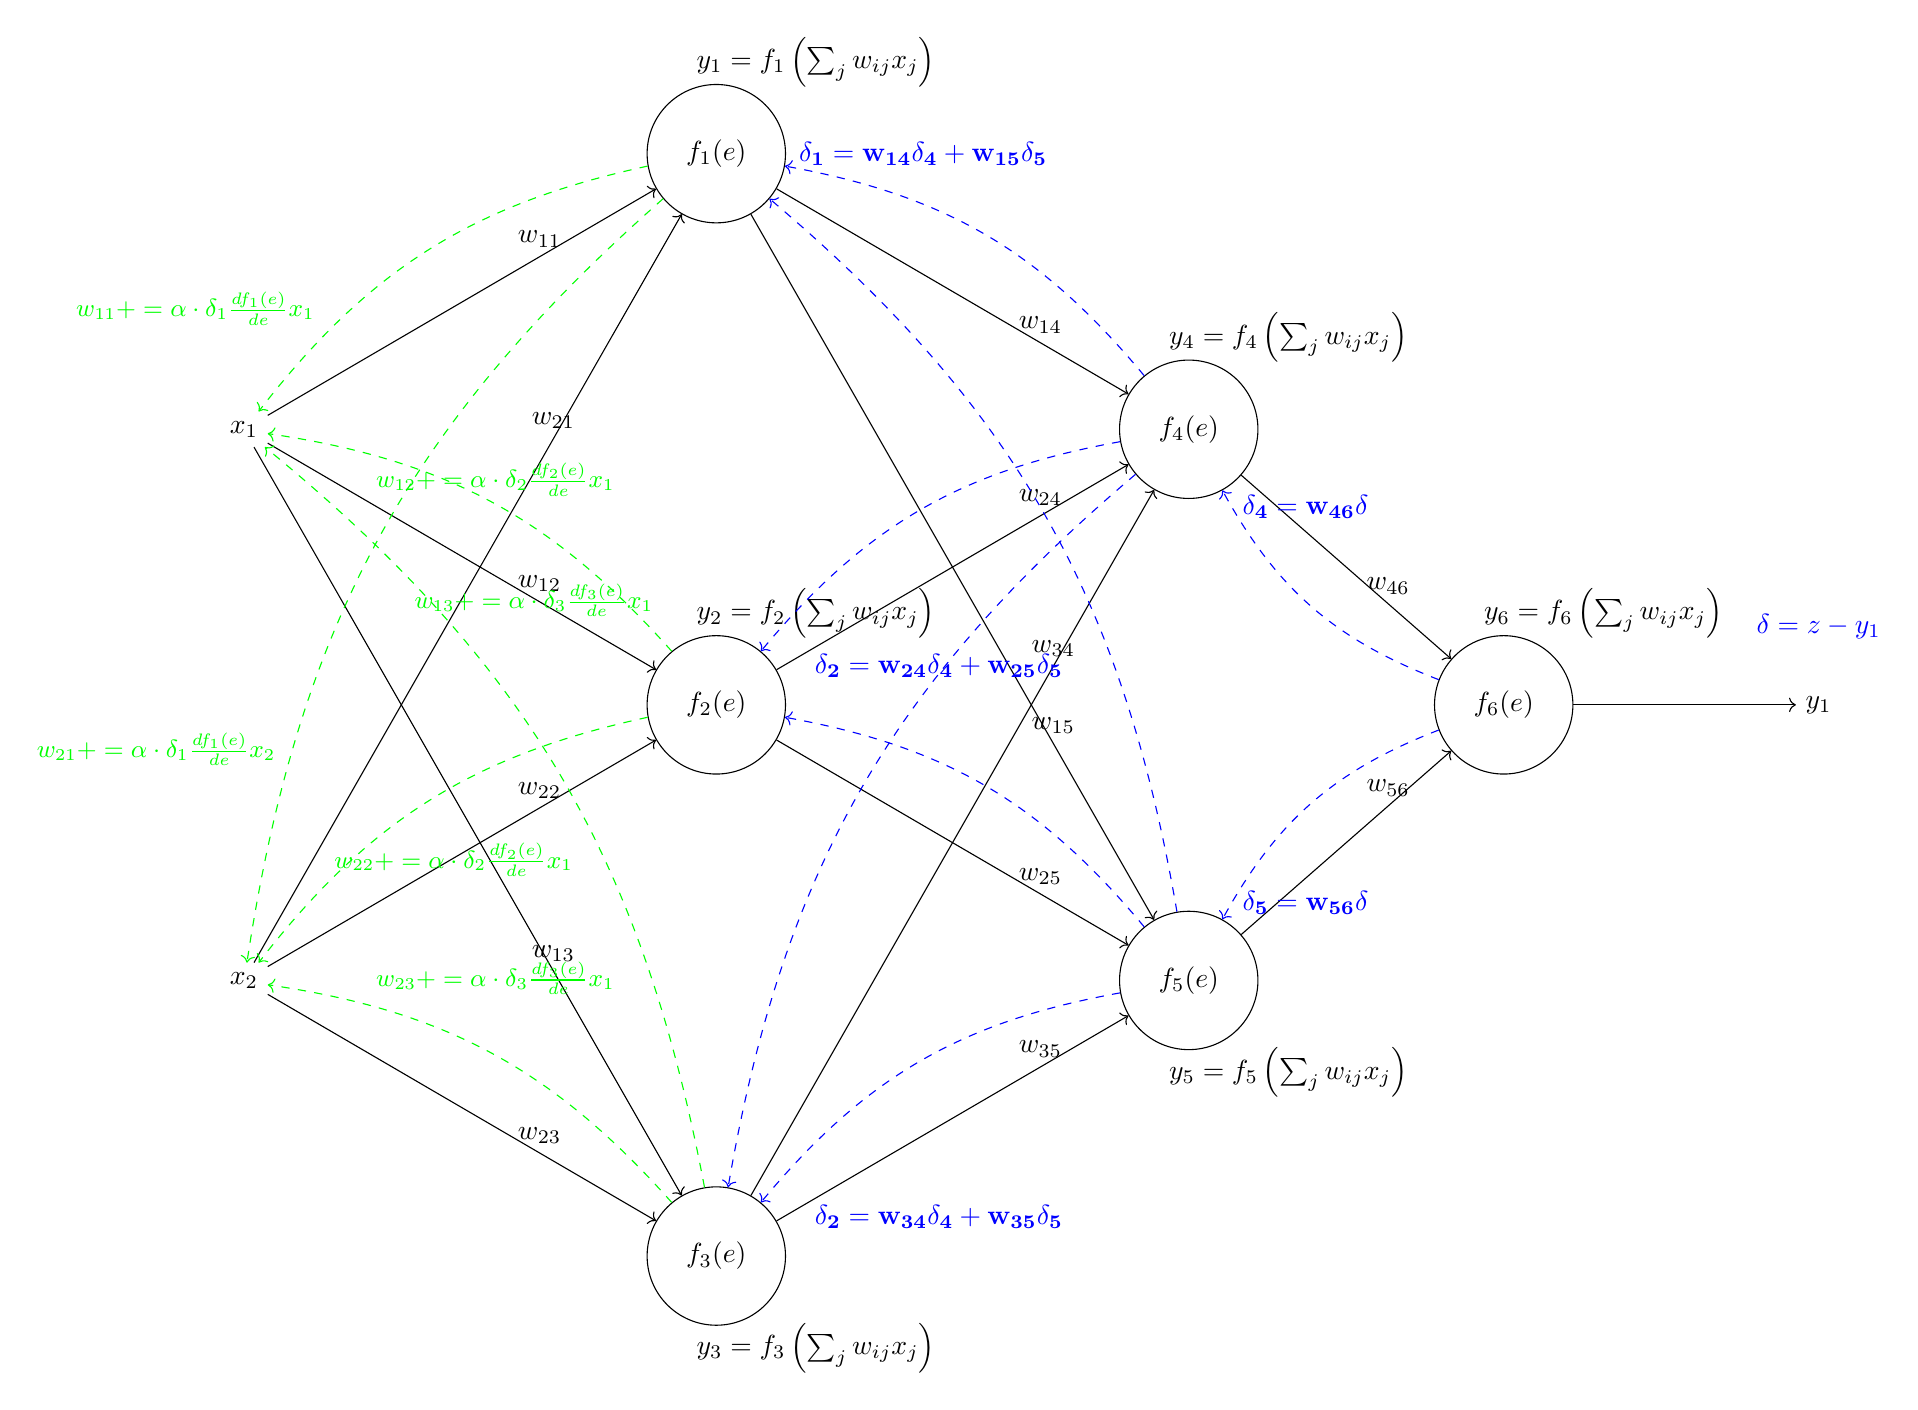
\begin{tikzpicture}
\tikzstyle{update}=[dashed, blue]
\tikzstyle{update2}=[dashed, green, font=\small]
\tikzstyle{neuron}=[circle,draw, minimum size=5em]
\usetikzlibrary{positioning}

%%%%%%%%%%%%%%%%%%%%%%%%%%%%%%
%%%%%%%%%%%%%%%%%%%%%%%%%%%%%%
%%%%%%%%%%%%%%%%%%%%%%%%%%%%%%
%%%%%%%%%%%%%%%%%%%%%%%%%%%%%%
%%%%%
%%%%% RED NEURONAL

%%%%% ENTRADA
\coordinate (x_1) at (-6, 3.5);
\coordinate (x_2) at (-6, -3.5);

%%%%% NEURONAS
\coordinate (f_1) at (0, 7);
\coordinate (f_2) at (0, 0);
\coordinate (f_3) at (0, -7);

\coordinate (f_4) at (6, 3.5);
\coordinate (f_5) at (6, -3.5);

\coordinate (f_6) at (10,0);

%%%%% SALIDA
\coordinate (y_1) at (14,0);


%%%%% CAPA ENTRADA
\node[] (x_1) at (x_1) {$x_1$};
\node[] (x_2) at (x_2) {$x_2$};

%%%%%%%%%%%%%%%
%%%%% CAPAS OCULTAS

%%%%% CAPA OCULTA 1
\node[neuron] (f_1) at (f_1) {$f_1(e)$};
\node[neuron] (f_2) at (f_2) {$f_2(e)$};
\node[neuron] (f_3) at (f_3) {$f_3(e)$};

%%%%% CAPA OCULTA 2
\node[neuron] (f_4) at (f_4) {$f_4(e)$};
\node[neuron] (f_5) at (f_5) {$f_5(e)$};

%%%%%%%%%%%%%%%
%%%%% CAPA SALIDA
\node[neuron] (f_6) at (f_6) {$f_6(e)$};
\node (y_1) at (y_1) {$y_1$};

%%%%%%%%%%%%%%%
%%%%% CONEXIONES
\draw[->] (x_1) -- node[above, pos=0.7] {$w_{11}$} (f_1);
\draw[->] (x_1) -- node[above, pos=0.7] {$w_{12}$} (f_2);
\draw[->] (x_1) -- node[above, pos=0.7] {$w_{13}$} (f_3);
\draw[->] (x_2) -- node[above, pos=0.7] {$w_{21}$} (f_1);
\draw[->] (x_2) -- node[above, pos=0.7] {$w_{22}$} (f_2);
\draw[->] (x_2) -- node[above, pos=0.7] {$w_{23}$} (f_3);


\draw[->] (f_1) -- node[above, pos=0.75] {$w_{14}$} (f_4);
\draw[->] (f_1) -- node[above, pos=0.75] {$w_{15}$} (f_5);
\draw[->] (f_2) -- node[above, pos=0.75] {$w_{24}$} (f_4);
\draw[->] (f_2) -- node[above, pos=0.75] {$w_{25}$} (f_5);
\draw[->] (f_3) -- node[above, pos=0.75] {$w_{34}$} (f_4);
\draw[->] (f_3) -- node[above, pos=0.75] {$w_{35}$} (f_5);

\draw[->] (f_4) -- node[above, pos=0.7] {$w_{46}$} (f_6);
\draw[->] (f_5) -- node[above, pos=0.7] {$w_{56}$} (f_6);


\draw[->] (f_6) --  (y_1);

%%%%%%%%%%%%%%%%%%%%%%%%%%%%%%
%%%%%%%%%%%%%%%%%%%%%%%%%%%%%%
%%%%%%%%%%%%%%%%%%%%%%%%%%%%%%
%%%%%%%%%%%%%%%%%%%%%%%%%%%%%%
%%%%%
%%%%% ENTRENAMIENTO
\newcommand{\f}[1]{${y_#1 = f_#1\left(\sum_{j} w_{ij}x_j\right)}$}
\node[above right = 0.1 and -1 of f_1,] {\f{1}};
\node[above right = 0.1 and -1 of f_2] {\f{2}};
\node[below right = 0.1 and -1 of f_3] {\f{3}};

\node[above right=0.1 and -1 of f_4] {\f{4}};
\node[below right=0.1 and -1 of f_5] {\f{5}};

\node[above right = 0.1 and -1 of f_6] {\f{6}};

%%%%%%%%%%%%%%%%%%%%%%%%%%%%%%
%%%%%%%%%%%%%%%%%%%%%%%%%%%%%%
%%%%%%%%%%%%%%%%%%%%%%%%%%%%%%
%%%%%%%%%%%%%%%%%%%%%%%%%%%%%%
%%%%%
%%%%% RETROPROPAGACIÓN
% CALCULO DEL ERROR
% http://stats.stackexchange.com/questions/94387/how-to-derive-errors-in-neural-network-with-the-backpropagation-algorithm
\node[update, above of= y_1] {$\delta = z - y_1$};

\draw[update, ->] (f_6) to [bend left=20] node[above right=1.0 and -1] {$\mathbf{\delta_4 = w_{46}\delta}$} (f_4);
\draw[update, ->] (f_6) to [bend left=-20] node[below right=1.0 and -1] {$\mathbf{\delta_5 = w_{56}\delta}$} (f_5);

\node[below right=-0.9 and 0.3 of f_1, blue] {$\mathbf{\delta_1 = w_{14}\delta_4 + w_{15}\delta_5}$};
\draw[update, ->] (f_4) to [bend left=-20] (f_1);
\draw[update, ->] (f_5) to [bend left=-20] (f_1);

\node[above right=-0.4 and 0.5 of f_2, blue] {$\mathbf{\delta_2 = w_{24}\delta_4 + w_{25}\delta_5}$};
\draw[update, ->] (f_4) to [bend left=-20] (f_2);
\draw[update, ->] (f_5) to [bend left=-20] (f_2);

\node[above right=-0.4 and 0.5 of f_3, blue] {$\mathbf{\delta_2 = w_{34}\delta_4 + w_{35}\delta_5}$};
\draw[update, ->] (f_4) to [bend left=-20] (f_3);
\draw[update, ->] (f_5) to [bend left=-20] (f_3);

%%%%%
%%%%% CALCULO DE LOS PESOS
% http://galaxy.agh.edu.pl/~vlsi/AI/backp_t_en/backprop.html
% https://theclevermachine.wordpress.com/tag/backpropagation/
\newcommand{\up}[4]{${#1 += \alpha\cdot#2\frac{d #3(e)}{de}#4}$}
\draw[update2, ->] (f_1) to [bend right=20] node[above left, pos=0.8] {\up{w_{11}}{\delta_1}{f_1}{x_1}} (x_1);
\draw[update2, ->] (f_1) to [bend right=20] node[above left, pos=0.8] {\up{w_{21}}{\delta_1}{f_1}{x_2}} (x_2);

\draw[update2, ->] (f_2) to [bend right=20] node[below right, pos=0.8] {\up{w_{12}}{\delta_2}{f_2}{x_1}} (x_1);
\draw[update2, ->] (f_2) to [bend right=20] node[above right, pos=0.8] {\up{w_{22}}{\delta_2}{f_2}{x_1}} (x_2);

\draw[update2, ->] (f_3) to [bend right=20] node[below right, pos=0.8] {\up{w_{13}}{\delta_3}{f_3}{x_1}} (x_1);
\draw[update2, ->] (f_3) to [bend right=20] node[above right, pos=0.8] {\up{w_{23}}{\delta_3}{f_3}{x_1}} (x_2);

\end{tikzpicture}
%!tikz source end

\end{document}}
    \end{figure}
\end{frame}

\begin{frame}{\titulo}{\subtitulo}
    \begin{itemize}
        \item Cuando se utiliza una red neural para aproximar una función, los datos se transmiten a través de la red, capa por capa, hasta llegar a la capa final.\bigskip

        \item La activación de la capa final corresponde a la predicción realizada por la red.\bigskip

        \item La clave es encontrar el conjunto adecuado de pesos para todas las conexiones.
    \end{itemize}
\end{frame}

\section{La función de costo}
\begin{frame}{\titulo}{\subtitulo}
    \begin{columns}
        \column{0.45\textwidth}
        \begin{itemize}
            \small
            \item Cuando se entrena la red, es conveniente tener alguna métrica de lo bueno o malo que estamos haciendo.

            \item Se denomina a esta métrica como {\bf función de coste} y denotaremos $J(W)$.\bigskip

            \item La diferencia entre los resultados de las estimaciones y los puntos de datos de entrenamiento son los valores principales de nuestra función de coste.\bigskip

            \item El objetivo será lograr que el valor de la función de coste sea lo más bajo posible .\bigskip

            \item La función de costo debe ser más o menos convexa
        \end{itemize}

        \column{0.5\textwidth}
        \begin{figure}[H]
            \includegraphics[scale=0.3]{img/convexa.png}
        \end{figure}
    \end{columns}
\end{frame}

%\begin{frame}{\titulo}{\subtitulo}
%    \begin{itemize}
        %\item En realidad, es imposible para cualquier red o función de costes sean verdaderamente convexa.\bigskip

        %\item Sin embargo, como veremos pronto, los mínimos locales pueden no ser un gran problema, siempre y cuando todavía hay una tendencia general que debemos seguir para llegar a la parte inferior.\bigskip

        %\item Además, observe que la función de coste es parametrizada por los pesos de nuestra red - controlamos nuestra función de pérdida cambiando los pesos.
    %\end{itemize}
%\end{frame}

\section{Minimizar la función de costo}
\begin{frame}{\titulo}{\subtitulo}
    \begin{itemize}
        \item Se deben encontrar los pesos que harán que la puntuación más baja posible.\bigskip

        \item La primera solución es derivar la función de coste e igualarla a cero, ásí se obtendría la ubicación de cada mínimo/máximo en la función.\bigskip

        \item Este intuitivo método tiene algunos problemas:
        \begin{enumerate}
            \item La función de costo no es una función simple, y el cálculo de su derivada no es sencillo.\medskip

            \item La función de costo es multidimensional (una dimensión por cada peso).\medskip

            \item Existe mas de un mínimo y máximo asociados a la función.
        \end{enumerate}
    \end{itemize}
\end{frame}

\section{El algoritmo de retropopagación}
\begin{frame}{\titulo}{\subtitulo}
    \begin{figure}[H]
        \centering
        %\scalebox{0.6}{% http://staff.itee.uq.edu.au/janetw/cmc/chapters/BackProp/index2.html
% http://outlace.com/Beginner-Tutorial-Backpropagation/
% http://neuralnetworksanddeeplearning.com/chap2.html
% http://staff.itee.uq.edu.au/janetw/cmc/chapters/BackProp/slides/Backprop_files/frame.htm
% http://staff.itee.uq.edu.au/janetw/cmc/chapters/BackProp/
% http://home.agh.edu.pl/~vlsi/AI/backp_t_en/backprop.html
% https://www.google.cl/webhp?sourceid=chrome-instant&ion=1&espv=2&ie=UTF-8#safe=off&q=backpropagation+practice+example
% https://ayearofai.com/rohan-4-the-vanishing-gradient-problem-ec68f76ffb9b#.9ntv81akz

\ifx\du\undefined
  \newlength{\du}
\fi
\newcommand{\nweigth}[2]{$W^{#1}_{#2} - \alpha\frac{\partial J}{\partial W^{#1}_{#2}}$}
\newcommand{\w}[2]{$W^{#1}_{#2}$}

\setlength{\du}{1\unitlength}
\begin{tikzpicture}[font=\small]
\tikzstyle{neuron}=[circle,draw, minimum size=2em]
\tikzstyle{update}=[dashed, blue]

\pgftransformxscale{1.000000}
\pgftransformyscale{-1.000000}

\coordinate (x1)    at (0.000000\du, 0.000000\du);
\coordinate (x2)    at (0.000000\du, 8.000000\du);

\coordinate (i)     at (3.000000\du, 0.000000\du);
\coordinate (ii)    at (3.000000\du, 8.000000\du);

\coordinate (iv)    at (10.000000\du, 0.000000\du);
\coordinate (v)     at (10.000000\du, 8.000000\du);

\coordinate (vii)   at (17.000000\du, 0.000000\du);
\coordinate (viii)  at (17.000000\du, 8.000000\du);

\coordinate (ix)   at (17.000000\du, 0.000000\du);
\coordinate (diez)  at (17.000000\du, 8.000000\du);


\coordinate (x)     at (24.000000\du, 4.000000\du);
\coordinate (y)     at (27.000000\du, 4.000000\du);


%%%%%%%%%%%%%%%%%%%%%%%%%%%%%%%%%%%%%%%%%%%%%%%%%%%%%%%%%%
% ENTRADA
\node (X1) at (x1) {\Huge $x_1$};
\node (X2) at (x2) {\Huge $x_2$};

% CAPA DE ENTRADA
\node[neuron] (A) at  (i) {}; % A
\node[neuron] (B) at  (ii)  {}; % B

% CAPA 1
\node[neuron] (C) at  (iv)  {}; % C
\node[neuron] (D) at  (v)  {}; % D

% CAPA 2
\node[neuron] (E) at  (vii)  {}; % E
\node[neuron] (F) at  (viii)  {}; % F

% CAPA 2
\node[neuron] (H) at  (ix)  {}; % E
\node[neuron] (I) at  (diez)  {}; % F

% CAPA DE SALIDA
\node[neuron] (G) at  (x)  {}; % G

% SALIDA
\node (out) at (y) {\Huge $y_1$};
%%%%%%%%%%%%%%%%%%%%%%%%%%%%%%%%%%%%%%%%%%%%%%%%%%%%%%%%%%


\draw[->] (X1) -- (A);
\draw[->] (X2) -- (B);


%%%%%%%%%%%%%%%%%%%%%%%%%%%%%%%%%%%%%%%%%%%%%%%%%%%%%%%%%%
%%%%%%%%%%%%%%%%%%%%%%%%%%%%%%%%%%%%%%%%%%%%%%%%%%%%%%%%%%
\draw[->] (A) -- node[above, pos=0.2] (W_1_11) {\w{1}{11}} (C);
\draw[->] (A) -- node[left , pos=0.2] (W_1_12) {\w{1}{12}} (D);
\draw[->] (B) -- node[left , pos=0.2] (W_1_13) {\w{1}{13}} (C);
\draw[->] (B) -- node[below, pos=0.2] (W_1_14) {\w{1}{14}} (D);

%\draw[->, dashed, blue] (C) to [bend left=40] node[above] {$W^{1}_{11} - \alpha\frac{\partial J}{\partial W^{1}_{11}}$} (W_1_11);
\draw[->, update] (C) to [bend left=40] node[above] {\nweigth{1}{11}} (W_1_11);
\draw[->, update] (D) to [bend left=50] node[above right, pos=0.98] {\nweigth{1}{12}} (W_1_12);

\draw[->, update] (C) to [bend right=50] node[below right, pos=0.98] {\nweigth{1}{13}} (W_1_13);
\draw[->, update] (D) to [bend right=40] node[below] {\nweigth{1}{14}} (W_1_14);

%%%%%%%%%%%%%%%%%%%%%%%%%%%%%%%%%%%%%%%%%%%%%%%%%%%%%%%%%%
%%%%%%%%%%%%%%%%%%%%%%%%%%%%%%%%%%%%%%%%%%%%%%%%%%%%%%%%%%
\draw[->] (C) -- node[above, pos=0.2] (W_2_11) {\w{l}{11}} (E);
\draw[->] (C) -- node[left , pos=0.2] (W_2_12) {\w{2}{12}} (F);
\draw[->] (D) -- node[left , pos=0.2] (W_2_13) {\w{2}{13}} (E);
\draw[->] (D) -- node[below, pos=0.2] (W_2_14) {\w{2}{14}} (F);

\draw[->, update] (E) to [bend left=40] node[above] {\nweigth{2}{11}} (W_2_11);
\draw[->, update] (F) to [bend left=50] node[above right, pos=0.98] {\nweigth{2}{12}} (W_2_12);

\draw[->, update] (E) to [bend right=50] node[below right, pos=0.98] {\nweigth{2}{13}} (W_2_13);
\draw[->, update] (F) to [bend right=40] node[below] {\nweigth{2}{14}} (W_2_14);

%%%%%%%%%%%%%%%%%%%%%%%%%%%%%%%%%%%%%%%%%%%%%%%%%%%%%%%%%%
%%%%%%%%%%%%%%%%%%%%%%%%%%%%%%%%%%%%%%%%%%%%%%%%%%%%%%%%%%
\draw[->] (E) -- node[right, pos=0.2] (W_3_11) {\w{3}{11}} (G);
\draw[->] (F) -- node[right, pos=0.2] (W_3_12) {\w{3}{12}} (G);

\draw[->, update] (G) to [bend  left=50] node[above right, pos=0.98] {\nweigth{3}{11}} (W_3_11);
\draw[->, update] (G) to [bend right=40] node[below right, pos=0.98] {\nweigth{3}{12}} (W_3_12);


\draw[->] (G) -- (out);
\end{tikzpicture}
}
        \scalebox{0.6}{% http://staff.itee.uq.edu.au/janetw/cmc/chapters/BackProp/index2.html
% http://outlace.com/Beginner-Tutorial-Backpropagation/
% http://neuralnetworksanddeeplearning.com/chap2.html
% http://staff.itee.uq.edu.au/janetw/cmc/chapters/BackProp/slides/Backprop_files/frame.htm
% http://staff.itee.uq.edu.au/janetw/cmc/chapters/BackProp/
% http://home.agh.edu.pl/~vlsi/AI/backp_t_en/backprop.html
% https://www.google.cl/webhp?sourceid=chrome-instant&ion=1&espv=2&ie=UTF-8#safe=off&q=backpropagation+practice+example
% https://ayearofai.com/rohan-4-the-vanishing-gradient-problem-ec68f76ffb9b#.9ntv81akz

\ifx\du\undefined
  \newlength{\du}
\fi
\newcommand{\nweigth}[2]{$W^{#1}_{#2} - \alpha\frac{\partial J}{\partial W^{#1}_{#2}}$}
\newcommand{\w}[2]{$W^{#1}_{#2}$}

\setlength{\du}{1\unitlength}
\begin{tikzpicture}[font=\small]
\tikzstyle{neuron}=[circle,draw, minimum size=2em]
\tikzstyle{update}=[dashed, blue]

\pgftransformxscale{1.000000}
\pgftransformyscale{-1.000000}

\coordinate (x1)    at (0.000000\du, 0.000000\du);
\coordinate (x2)    at (0.000000\du, 8.000000\du);

\coordinate (i)     at (3.000000\du, 0.000000\du);
\coordinate (ii)    at (3.000000\du, 8.000000\du);

\coordinate (iv)    at (10.000000\du, 0.000000\du);
\coordinate (v)     at (10.000000\du, 8.000000\du);

\coordinate (vii)   at (17.000000\du, 0.000000\du);
\coordinate (viii)  at (17.000000\du, 8.000000\du);

\coordinate (ix)   at (17.000000\du, 0.000000\du);
\coordinate (diez)  at (17.000000\du, 8.000000\du);


\coordinate (x)     at (24.000000\du, 4.000000\du);
\coordinate (y)     at (27.000000\du, 4.000000\du);


%%%%%%%%%%%%%%%%%%%%%%%%%%%%%%%%%%%%%%%%%%%%%%%%%%%%%%%%%%
% ENTRADA
\node (X1) at (x1) {\Huge $x_1$};
\node (X2) at (x2) {\Huge $x_2$};

% CAPA DE ENTRADA
\node[neuron] (A) at  (i) {}; % A
\node[neuron] (B) at  (ii)  {}; % B

% CAPA 1
\node[neuron] (C) at  (iv)  {}; % C
\node[neuron] (D) at  (v)  {}; % D

% CAPA 2
\node[neuron] (E) at  (vii)  {}; % E
\node[neuron] (F) at  (viii)  {}; % F

% CAPA 2
\node[neuron] (H) at  (ix)  {}; % E
\node[neuron] (I) at  (diez)  {}; % F

% CAPA DE SALIDA
\node[neuron] (G) at  (x)  {}; % G

% SALIDA
\node (out) at (y) {\Huge $y_1$};
%%%%%%%%%%%%%%%%%%%%%%%%%%%%%%%%%%%%%%%%%%%%%%%%%%%%%%%%%%


\draw[->] (X1) -- (A);
\draw[->] (X2) -- (B);


%%%%%%%%%%%%%%%%%%%%%%%%%%%%%%%%%%%%%%%%%%%%%%%%%%%%%%%%%%
%%%%%%%%%%%%%%%%%%%%%%%%%%%%%%%%%%%%%%%%%%%%%%%%%%%%%%%%%%
\draw[->] (A) -- node[above, pos=0.2] (W_1_11) {\w{1}{11}} (C);
\draw[->] (A) -- node[left , pos=0.2] (W_1_12) {\w{1}{12}} (D);
\draw[->] (B) -- node[left , pos=0.2] (W_1_13) {\w{1}{13}} (C);
\draw[->] (B) -- node[below, pos=0.2] (W_1_14) {\w{1}{14}} (D);

%\draw[->, dashed, blue] (C) to [bend left=40] node[above] {$W^{1}_{11} - \alpha\frac{\partial J}{\partial W^{1}_{11}}$} (W_1_11);
\draw[->, update] (C) to [bend left=40] node[above] {\nweigth{1}{11}} (W_1_11);
\draw[->, update] (D) to [bend left=50] node[above right, pos=0.98] {\nweigth{1}{12}} (W_1_12);

\draw[->, update] (C) to [bend right=50] node[below right, pos=0.98] {\nweigth{1}{13}} (W_1_13);
\draw[->, update] (D) to [bend right=40] node[below] {\nweigth{1}{14}} (W_1_14);

%%%%%%%%%%%%%%%%%%%%%%%%%%%%%%%%%%%%%%%%%%%%%%%%%%%%%%%%%%
%%%%%%%%%%%%%%%%%%%%%%%%%%%%%%%%%%%%%%%%%%%%%%%%%%%%%%%%%%
\draw[->] (C) -- node[above, pos=0.2] (W_2_11) {\w{l}{11}} (E);
\draw[->] (C) -- node[left , pos=0.2] (W_2_12) {\w{2}{12}} (F);
\draw[->] (D) -- node[left , pos=0.2] (W_2_13) {\w{2}{13}} (E);
\draw[->] (D) -- node[below, pos=0.2] (W_2_14) {\w{2}{14}} (F);

\draw[->, update] (E) to [bend left=40] node[above] {\nweigth{2}{11}} (W_2_11);
\draw[->, update] (F) to [bend left=50] node[above right, pos=0.98] {\nweigth{2}{12}} (W_2_12);

\draw[->, update] (E) to [bend right=50] node[below right, pos=0.98] {\nweigth{2}{13}} (W_2_13);
\draw[->, update] (F) to [bend right=40] node[below] {\nweigth{2}{14}} (W_2_14);

%%%%%%%%%%%%%%%%%%%%%%%%%%%%%%%%%%%%%%%%%%%%%%%%%%%%%%%%%%
%%%%%%%%%%%%%%%%%%%%%%%%%%%%%%%%%%%%%%%%%%%%%%%%%%%%%%%%%%
\draw[->] (E) -- node[right, pos=0.2] (W_3_11) {\w{3}{11}} (G);
\draw[->] (F) -- node[right, pos=0.2] (W_3_12) {\w{3}{12}} (G);

\draw[->, update] (G) to [bend  left=50] node[above right, pos=0.98] {\nweigth{3}{11}} (W_3_11);
\draw[->, update] (G) to [bend right=40] node[below right, pos=0.98] {\nweigth{3}{12}} (W_3_12);


\draw[->] (G) -- (out);
\end{tikzpicture}
}
    \end{figure}
\end{frame}

\subsection{El gradiente descendente}
\begin{frame}{\titulo}{\subtitulo}
    \begin{itemize}
        \item Como el tamaño de las redes comienza a ampliar, la solución para los pesos se convierte directamente cada vez inviable.\bigskip

        \item En su lugar, nos fijamos en una clase diferente de algoritmos, llamados algoritmos de optimización iterativos, que funciona progresivamente su camino hacia la solución óptima.\bigskip

        \item El más básico de estos algoritmos es el de gradiente descendente.\bigskip

        \item Recordemos que nuestra función de coste será esencialmente convexa, y queremos llegar lo más cerca posible del mínimo global.\bigskip

        \item En lugar de resolver analíticamente, el gradiente descendente sigue los derivados esencialmente a "rodar" por la pendiente hasta que encuentra su camino hacia el centro.
    \end{itemize}
\end{frame}

\begin{frame}{\titulo}{\subtitulo}
    \begin{itemize}
        \item Tomemos una red neuronal de un solo peso, cuya función de costes se representa a continuación.
        \begin{figure}[H]
            \includegraphics[scale=0.15]{img/gd1.png}
        \end{figure}

        \item Comenzamos por la inicialización de nuestro peso al azar, lo que nos sitúa en el punto rojo en el diagrama anterior.\bigskip

        \item Tomando la derivada, vemos la pendiente en este punto es un número positivo muy grande.\bigskip

        \item Queremos ir más cerca del centro, para eso hay que tomar un paso bastante grande en la dirección opuesta de la pendiente.
    \end{itemize}
\end{frame}

\begin{frame}{\titulo}{\subtitulo}
    \begin{itemize}
        \footnotesize
        \item Si repetimos el proceso lo suficiente, pronto nos encontramos casi en la parte inferior de nuestra curva y mucho más cerca de la configuración óptima del peso de nuestra red.
        \begin{figure}[H]
            \includegraphics[scale=0.15]{img/gd2.png}
        \end{figure}

        \item Más formalmente, el gradiente descendente se describe como sigue $$ W = W - \alpha\frac{\partial J}{\partial W} $$

        \item Para actualizar el peso se le resta la derivada de la función de coste escalada por una tasa de aprendizaje.\bigskip

        \item Usted verá que a medida que se acerca cada vez más cerca del centro, el término derivado se hace más pequeña, que converge a cero al aproximarse a la solución.\bigskip

        \item El mismo proceso se aplica con redes que tienen decenas, cientos, miles o más parámetros.
    \end{itemize}
\end{frame}

\begin{frame}{\titulo}{\subtitulo}
    \begin{itemize}
        %\item Yo quiero decir unas pocas palabras más sobre la tasa de aprendizaje, porque es uno de los más importantes hiperparamétrico que usted tiene control sobre.\bigskip

        \item Si la tasa de aprendizaje es demasiado alta, podría saltar demasiado lejos en la otra dirección, y nunca llegar al mínimo que está buscando.\bigskip

        \item Establece demasiado bajo, y su red se llevará a las edades para encontrar los pesos adecuados, o puede quedar atrapado en un mínimo local.\bigskip

        \item No hay "número mágico", para usar cuando se trata de una tasa de aprendizaje, y por lo general es mejor que probar varios y escoger el que funciona mejor para su red y conjunto de datos individual.\bigskip

        \item En la práctica, muchos optan por recocer la tasa de aprendizaje en el tiempo - que comienza alta, porque es más alejado de la solución, y se desintegra ya que se acerca.
    \end{itemize}
\end{frame}

\subsection{El desvanecimiento del gradiente}
\begin{frame}{\titulo}{\subtitulo}
	\begin{figure}[H]
        \centering
        %\scalebox{0.6}{% http://staff.itee.uq.edu.au/janetw/cmc/chapters/BackProp/index2.html
% http://outlace.com/Beginner-Tutorial-Backpropagation/
% http://neuralnetworksanddeeplearning.com/chap2.html
% http://staff.itee.uq.edu.au/janetw/cmc/chapters/BackProp/slides/Backprop_files/frame.htm
% http://staff.itee.uq.edu.au/janetw/cmc/chapters/BackProp/
% http://home.agh.edu.pl/~vlsi/AI/backp_t_en/backprop.html
% https://www.google.cl/webhp?sourceid=chrome-instant&ion=1&espv=2&ie=UTF-8#safe=off&q=backpropagation+practice+example
% https://ayearofai.com/rohan-4-the-vanishing-gradient-problem-ec68f76ffb9b#.9ntv81akz

\ifx\du\undefined
  \newlength{\du}
\fi
\newcommand{\nweigth}[2]{$W^{#1}_{#2} - \alpha\frac{\partial J}{\partial W^{#1}_{#2}}$}
\newcommand{\w}[2]{$W^{#1}_{#2}$}

\setlength{\du}{1\unitlength}
\begin{tikzpicture}[font=\small]
\tikzstyle{neuron}=[circle,draw, minimum size=2em]
\tikzstyle{update}=[dashed, blue]

\pgftransformxscale{1.000000}
\pgftransformyscale{-1.000000}

\coordinate (x1)    at (0.000000\du, 0.000000\du);
\coordinate (x2)    at (0.000000\du, 8.000000\du);

\coordinate (i)     at (3.000000\du, 0.000000\du);
\coordinate (ii)    at (3.000000\du, 8.000000\du);

\coordinate (iv)    at (10.000000\du, 0.000000\du);
\coordinate (v)     at (10.000000\du, 8.000000\du);

\coordinate (vii)   at (17.000000\du, 0.000000\du);
\coordinate (viii)  at (17.000000\du, 8.000000\du);

\coordinate (ix)   at (17.000000\du, 0.000000\du);
\coordinate (diez)  at (17.000000\du, 8.000000\du);


\coordinate (x)     at (24.000000\du, 4.000000\du);
\coordinate (y)     at (27.000000\du, 4.000000\du);


%%%%%%%%%%%%%%%%%%%%%%%%%%%%%%%%%%%%%%%%%%%%%%%%%%%%%%%%%%
% ENTRADA
\node (X1) at (x1) {\Huge $x_1$};
\node (X2) at (x2) {\Huge $x_2$};

% CAPA DE ENTRADA
\node[neuron] (A) at  (i) {}; % A
\node[neuron] (B) at  (ii)  {}; % B

% CAPA 1
\node[neuron] (C) at  (iv)  {}; % C
\node[neuron] (D) at  (v)  {}; % D

% CAPA 2
\node[neuron] (E) at  (vii)  {}; % E
\node[neuron] (F) at  (viii)  {}; % F

% CAPA 2
\node[neuron] (H) at  (ix)  {}; % E
\node[neuron] (I) at  (diez)  {}; % F

% CAPA DE SALIDA
\node[neuron] (G) at  (x)  {}; % G

% SALIDA
\node (out) at (y) {\Huge $y_1$};
%%%%%%%%%%%%%%%%%%%%%%%%%%%%%%%%%%%%%%%%%%%%%%%%%%%%%%%%%%


\draw[->] (X1) -- (A);
\draw[->] (X2) -- (B);


%%%%%%%%%%%%%%%%%%%%%%%%%%%%%%%%%%%%%%%%%%%%%%%%%%%%%%%%%%
%%%%%%%%%%%%%%%%%%%%%%%%%%%%%%%%%%%%%%%%%%%%%%%%%%%%%%%%%%
\draw[->] (A) -- node[above, pos=0.2] (W_1_11) {\w{1}{11}} (C);
\draw[->] (A) -- node[left , pos=0.2] (W_1_12) {\w{1}{12}} (D);
\draw[->] (B) -- node[left , pos=0.2] (W_1_13) {\w{1}{13}} (C);
\draw[->] (B) -- node[below, pos=0.2] (W_1_14) {\w{1}{14}} (D);

%\draw[->, dashed, blue] (C) to [bend left=40] node[above] {$W^{1}_{11} - \alpha\frac{\partial J}{\partial W^{1}_{11}}$} (W_1_11);
\draw[->, update] (C) to [bend left=40] node[above] {\nweigth{1}{11}} (W_1_11);
\draw[->, update] (D) to [bend left=50] node[above right, pos=0.98] {\nweigth{1}{12}} (W_1_12);

\draw[->, update] (C) to [bend right=50] node[below right, pos=0.98] {\nweigth{1}{13}} (W_1_13);
\draw[->, update] (D) to [bend right=40] node[below] {\nweigth{1}{14}} (W_1_14);

%%%%%%%%%%%%%%%%%%%%%%%%%%%%%%%%%%%%%%%%%%%%%%%%%%%%%%%%%%
%%%%%%%%%%%%%%%%%%%%%%%%%%%%%%%%%%%%%%%%%%%%%%%%%%%%%%%%%%
\draw[->] (C) -- node[above, pos=0.2] (W_2_11) {\w{l}{11}} (E);
\draw[->] (C) -- node[left , pos=0.2] (W_2_12) {\w{2}{12}} (F);
\draw[->] (D) -- node[left , pos=0.2] (W_2_13) {\w{2}{13}} (E);
\draw[->] (D) -- node[below, pos=0.2] (W_2_14) {\w{2}{14}} (F);

\draw[->, update] (E) to [bend left=40] node[above] {\nweigth{2}{11}} (W_2_11);
\draw[->, update] (F) to [bend left=50] node[above right, pos=0.98] {\nweigth{2}{12}} (W_2_12);

\draw[->, update] (E) to [bend right=50] node[below right, pos=0.98] {\nweigth{2}{13}} (W_2_13);
\draw[->, update] (F) to [bend right=40] node[below] {\nweigth{2}{14}} (W_2_14);

%%%%%%%%%%%%%%%%%%%%%%%%%%%%%%%%%%%%%%%%%%%%%%%%%%%%%%%%%%
%%%%%%%%%%%%%%%%%%%%%%%%%%%%%%%%%%%%%%%%%%%%%%%%%%%%%%%%%%
\draw[->] (E) -- node[right, pos=0.2] (W_3_11) {\w{3}{11}} (G);
\draw[->] (F) -- node[right, pos=0.2] (W_3_12) {\w{3}{12}} (G);

\draw[->, update] (G) to [bend  left=50] node[above right, pos=0.98] {\nweigth{3}{11}} (W_3_11);
\draw[->, update] (G) to [bend right=40] node[below right, pos=0.98] {\nweigth{3}{12}} (W_3_12);


\draw[->] (G) -- (out);
\end{tikzpicture}
}
        \scalebox{0.6}{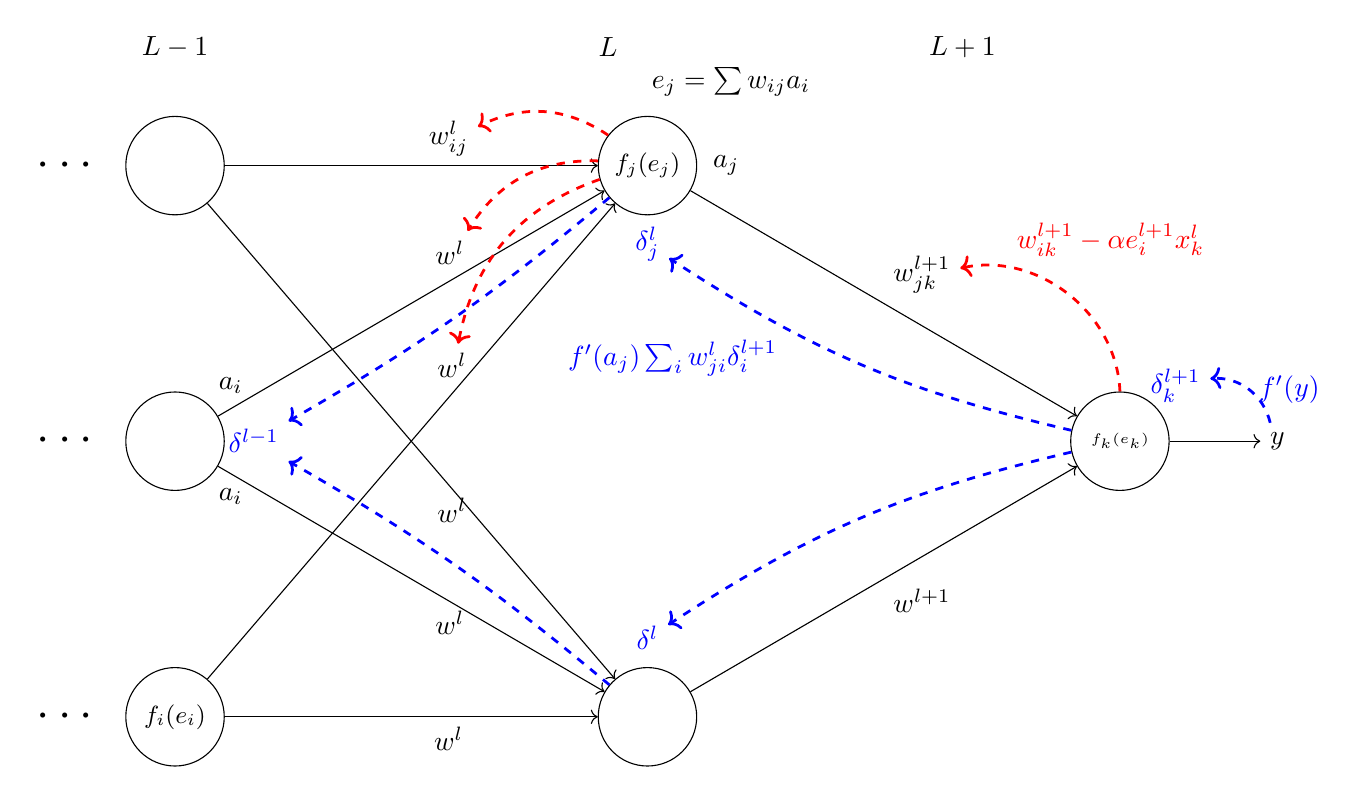
\begin{tikzpicture}

	\tikzstyle{nodo}=[circle, draw, minimum size=1.25cm]
	\tikzstyle{upw}=[dashed, red, ->, line width = 1pt]

	\coordinate (l_0) at (0, 5.0);
	\coordinate (l_1) at (5.5, 5.0);
	\coordinate (l_2) at (10, 5.0);

	\coordinate (f_1_1) at (0, 3.5); % CAPA ENTRADA
	\coordinate (f_1_2) at (0, 0); % CAPA ENTRADA
	\coordinate (f_1_3) at (0, -3.5); % CAPA ENTRADA
	\coordinate (f_2_1) at (6.0, 3.5); % CAPA OCULTA 1
	\coordinate (f_2_2) at (6.0, -3.5); % CAPA OCULTA 1
	\coordinate (f_3_1) at (12, 0); % CAPA SALIDA
	\coordinate (y) at (14, 0); % CAPA SALIDA

	\node[] (l_0) at (l_0) {$L - 1$};
	\node[] (l_1) at (l_1) {$L$};
	\node[] (l_2) at (l_2) {$L + 1$};

	\node[nodo] (f_1_1) at (f_1_1) {}; % CAPA ENTRADA
	\node[nodo] (f_1_2) at (f_1_2) {}; % CAPA ENTRADA
	\node[nodo] (f_1_3) at (f_1_3) {\small $f_i(e_i)$}; % CAPA ENTRADA
	\node[nodo] (f_2_1) at (f_2_1) {\small $f_j(e_j)$}; % CAPA OCULTA 1
	\node[nodo] (f_2_2) at (f_2_2) {}; % CAPA OCULTA 1
	\node[nodo] (f_3_1) at (f_3_1) {\tiny $f_k(e_k)$}; % CAPA SALIDA
	\node[] (y) at (y) {$y$}; % CAPA SALIDA

	\node[left of=f_1_1, node distance=1.4cm] {\LARGE $\cdots$};
	\node[left of=f_1_2, node distance=1.4cm] {\LARGE $\cdots$};
	\node[left of=f_1_3, node distance=1.4cm] {\LARGE $\cdots$};

	\draw[->] (f_1_1) -- node[pos=0.6, above] (w_1_1) {$w^{l}_{ij}$} (f_2_1);
	\draw[->] (f_1_2) -- node[pos=0.6, above] (w_1_2) {$w^{l}_{}$} (f_2_1);
	\draw[->] (f_1_3) -- node[pos=0.6, above] (w_1_3) {$w^{l}_{}$} (f_2_1);
	\draw[->] (f_1_1) node[above right of=f_1_2] {$a_{i}$} -- node[pos=0.6, below] (w_2_1) {$w^{l}_{}$} (f_2_2);
	\draw[->] (f_1_2) node[below right of=f_1_2] {$a_{i}$} -- node[pos=0.6, below] (w_2_2) {$w^{l}_{}$} (f_2_2);
	\draw[->] (f_1_3) -- node[pos=0.6, below] (w_2_3) {$w^{l}_{}$} (f_2_2);
	\draw[->] (f_2_1) node[right of=f_2_1] {$a_{j}$} -- node[pos=0.5, above right] (w_j_k) {$w^{l+1}_{jk}$} (f_3_1);
	\draw[->] (f_2_2) -- node[pos=0.5, below right] {$w^{l+1}$} (f_3_1);
	\draw[->] (f_3_1) -- node[pos=0.5, below right] {$$} (y);

	\node[above right of=f_2_1, node distance=1.5cm] {$e_{j} = \sum w_{ij}a_i$};


	\draw[upw] (f_3_1) to[bend right=50] node[above right, pos=0.8] {$w^{l+1}_{ik} - \alpha e^{l+1}_{i}x^{l}_{k}$} (w_j_k);
	\draw[upw] (f_2_1) to[bend right=30] node[above]{$$} (w_1_1);
	\draw[upw] (f_2_1) to[bend right=30] node[above]{$$} (w_1_2);
	\draw[upw] (f_2_1) to[bend right=30] node[above]{$$} (w_1_3);


	\node[blue, above right of=f_3_1] (e_i) {$\delta^{l+1}_{k}$};
	\node[blue, below of=f_2_1] (e_2_1_i) {$\delta^{l}_{j}$};
	\node[blue, above of=f_2_2] (e_2_2_i) {$\delta^{l}$};
	\node[blue, right of=f_1_2] (e_1_2_i) {$\delta^{l-1}$};

	\draw[upw, blue] (y) to[bend right=40] node[right]{$f'(y)$} (e_i);
	\draw[upw, blue] (f_3_1) to[bend left=10] node[below left, pos=0.7]{$f'(a_{j})\sum_{i}w^{l}_{ji}\delta^{l+1}_{i}$} (e_2_1_i);
	\draw[upw, blue] (f_3_1) to[bend right=10] (e_2_2_i);

	\draw[upw, blue] (f_2_1) to[bend left=5] (e_1_2_i);
	\draw[upw, blue] (f_2_2) to[bend right=5] (e_1_2_i);

\end{tikzpicture}
}
    \end{figure}
\end{frame}

\begin{frame}{\titulo}{\subtitulo}
\end{frame}

%\section{Actualización de los pesos}
%\begin{frame}{\titulo}{\subtitulo}
%    \begin{figure}[H]
%        \centering
%        \scalebox{0.55}{%!tikz editor 1.0
\documentclass{article}
\usepackage{tikz}
\usepackage[graphics, active, tightpage]{preview}
\PreviewEnvironment{tikzpicture}

%!tikz preamble begin
\usetikzlibrary{shapes,snakes}

%!tikz preamble end


\begin{document}
%!tikz source begin
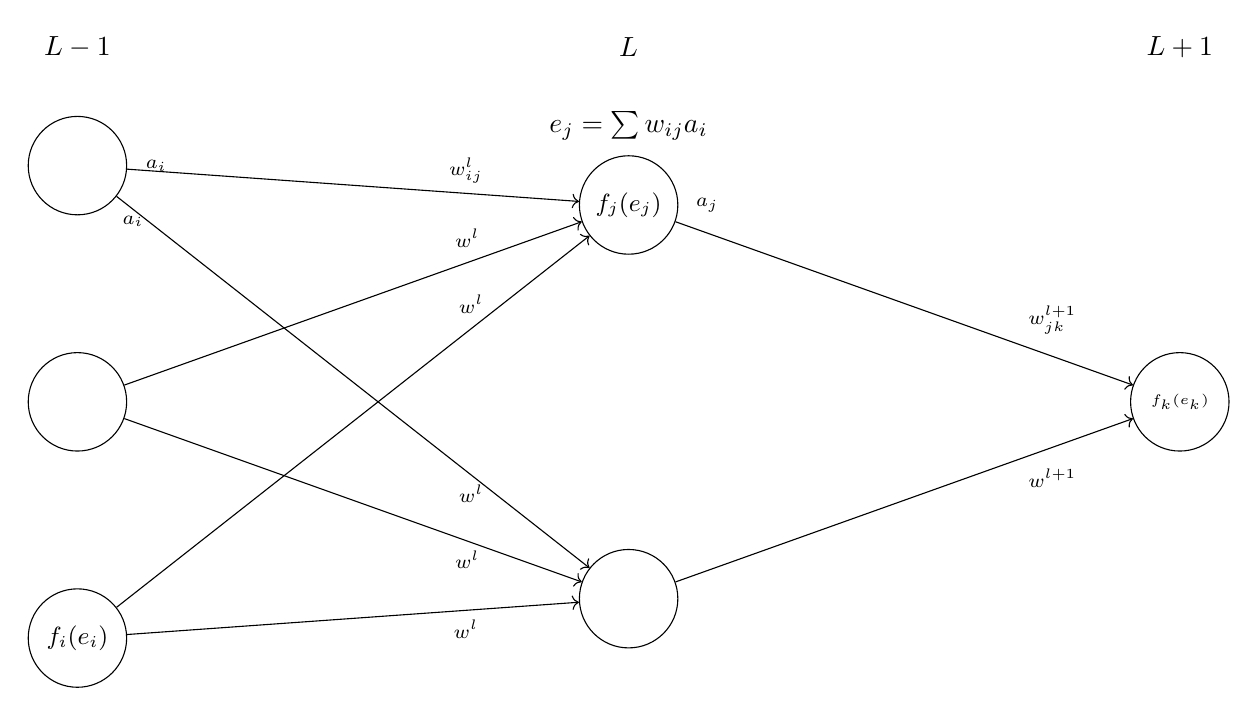
\begin{tikzpicture}
\tikzstyle{nodo}=[circle, draw, minimum size=1.25cm]
\tikzstyle{upw}=[dashed, red, ->, line width = 1pt]

\coordinate (l_0) at (0, 4.5);
\coordinate (l_1) at (7, 4.5);
\coordinate (l_2) at (14, 4.5);

\coordinate (f_1_1) at (0, 3); % CAPA ENTRADA
\coordinate (f_1_2) at (0, 0); % CAPA ENTRADA
\coordinate (f_1_3) at (0, -3); % CAPA ENTRADA
\coordinate (f_2_1) at (7, 2.5); % CAPA OCULTA 1
\coordinate (f_2_2) at (7, -2.5); % CAPA OCULTA 1
\coordinate (f_3_1) at (14, 0); % CAPA SALIDA

\node[] (l_0) at (l_0) {$L - 1$};
\node[] (l_1) at (l_1) {$L$};
\node[] (l_2) at (l_2) {$L + 1$};

\node[nodo] (f_1_1) at (f_1_1) {}; % CAPA ENTRADA
\node[nodo] (f_1_2) at (f_1_2) {}; % CAPA ENTRADA
\node[nodo] (f_1_3) at (f_1_3) {\small $f_i(e_i)$}; % CAPA ENTRADA
\node[nodo] (f_2_1) at (f_2_1) {\small $f_j(e_j)$}; % CAPA OCULTA 1
\node[nodo] (f_2_2) at (f_2_2) {}; % CAPA OCULTA 1
\node[nodo] (f_3_1) at (f_3_1) {\tiny $f_k(e_k)$}; % CAPA SALIDA


\draw[->, font=\scriptsize] (f_1_1) node[right of=f_1_1] {$a_{i}$} -- node[pos=0.75, above] (w_1_1) {$w^{l}_{ij}$} (f_2_1);
\draw[->, font=\scriptsize] (f_1_2) node[below right of=f_1_1] {$a_{i}$} -- node[pos=0.75, above] (w_1_2) {$w^{l}_{}$} (f_2_1);
\draw[->, font=\scriptsize] (f_1_3) -- node[pos=0.75, above] (w_1_3) {\scriptsize$w^{l}_{}$} (f_2_1);
\draw[->, font=\scriptsize] (f_1_1) -- node[pos=0.75, below] (w_2_1) {$w^{l}_{}$} (f_2_2);
\draw[->, font=\scriptsize] (f_1_2) -- node[pos=0.75, below] (w_2_2) {$w^{l}_{}$} (f_2_2);
\draw[->, font=\scriptsize] (f_1_3) -- node[pos=0.75, below] (w_2_3) {$w^{l}_{}$} (f_2_2);

\node[above of=f_2_1] {$e_{j} = \sum w_{ij}a_i$};

\draw[->, font=\scriptsize] (f_2_1) node[right of=f_2_1] {$a_{j}$} -- node[pos=0.75, above right] (w_j_k) {$w^{l+1}_{jk}$} (f_3_1);
\draw[->, font=\scriptsize] (f_2_2) -- node[pos=0.75, below right] {$w^{l+1}$} (f_3_1);
 
 
%\draw[upw] (f_3_1) to[bend left=20] (w_1_1);
%\draw[upw] (f_3_1) to[bend left=20] (w_1_2);
%\draw[upw] (f_3_1) to[bend left=20] node[pos=0.7, right] {$w^{l}_{ij} - \alpha\frac{\partial e}{\partial w}$} (w_1_3);


%\draw[upw] (f_4_1) to[bend right=20] node[pos=0.8, right] {$w^{l+1}_{jk} - \alpha\frac{\partial e}{\partial w^{l+1}_{jk}}$} (w_j_k);

%\node[above right of=w_j_k, node distance=3cm] {$\frac{\partial e}{\partial w^{l+1}_{jk}}=-(s_i - y_i)\frac{\partial y_i}{\partial w^{l+1}_{jk}}$};

\end{tikzpicture}
%!tikz source end

\end{document}}
%    \end{figure}
%
%    \begin{itemize}
%        \item $W^{l}_{ij}$ es el peso de la conexión entre la neurona $i$ de la capa $l$ con la neurona $j$ de la capa $l + 1$.
%    \end{itemize}
%\end{frame}
%
%\section{El algoritmo de retropropagación}
%\begin{frame}{\titulo}{\subtitulo}
%    \begin{itemize}
%        \item Para cualquier problema de aprendizaje supervisado queremos encontrar un conjunto de pesos $W$ que minimice la salida de $J(W)$.\bigskip
%
%        \item Cada neurona es una función de la neurona anterior conectada a ella.
%
%        \item Si uno cambiara el valor de $w_1$, las neuronas "ocultas 1" y "ocultas 2" cambiarían.
%
%        \item Debido a esta noción de dependencias funcionales, podemos formular matemáticamente el resultado como una función compuesta extensa:
%        \begin{eqnarray*}
%            output &=&  act(w_3*h_2)\\
%            h_2 &=&     act(w_2*h_1)\\
%            h_1 &=&     act(w_1*input)\\
%            &\Downarrow&\\
%            output &=&  act(w_3*act(w_2*act(w_1*input)))
%        \end{eqnarray*}
%
%        \item La salida es una función compuesta de los pesos, entradas y funciónes de activación.
%    \end{itemize}
%\end{frame}

%\begin{frame}{\titulo}{\subtitulo}
%\begin{itemize}
%    \item Si tomáramos entonces la derivada de dicha función con respecto a algún peso arbitrario, aplicaríamos iterativamente la regla de la cadena. El resultado sería similar al siguiente
%    \begin{eqnarray*}
%    \frac{\partial output}{\partial w_1}
%    =
%    \frac{\partial output}{\partial h_2}
%    \frac{\partial h_2}{\partial h_1}
%    \frac{\partial h_1}{\partial w_1}
%    \end{eqnarray*}
%
%    \item Ahora, vamos a adjuntar una caja negra a la cola de nuestra red neuronal. Esta caja negra calculará y devolverá el error - usando la función de coste - de nuestra salida
%    \begin{figure}[H]
%        \centering
%        \scalebox{0.55}{% http://home.agh.edu.pl/~vlsi/AI/backp_t_en/backprop.html
% http://home.agh.edu.pl/~vlsi/AI/backp_t_en/backprop.html
%\ifx\du\undefined
%  \newlength{\du}
%\fi
%\newcommand{\nweigth}[2]{$W^{#1}_{#2} - \alpha\frac{\partial J}{\partial W^{#1}_{#2}}$}
%\newcommand{\w}[2]{$W^{#1}_{#2}$}

%\setlength{\du}{15\unitlength}
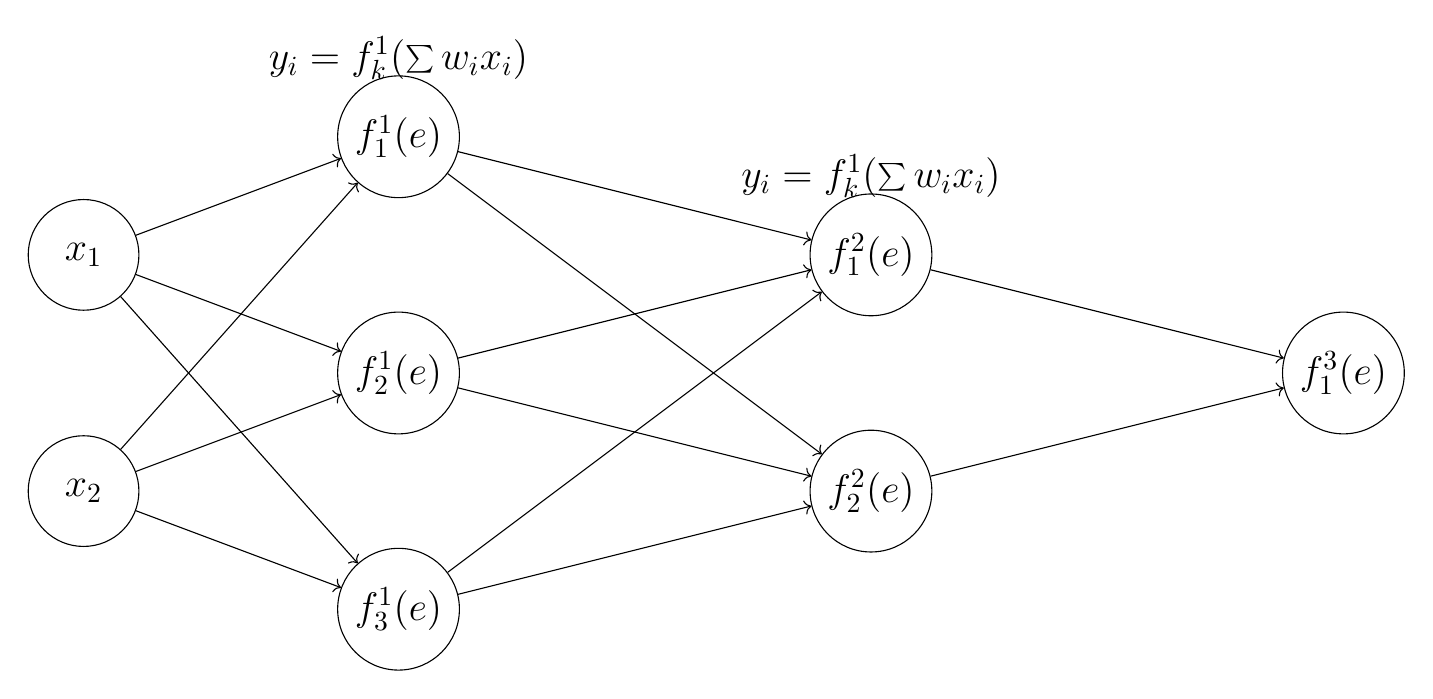
\begin{tikzpicture}
\tikzstyle{neuron}=[circle,draw, minimum size=4em, font=\Large]
\tikzstyle{update}=[dashed, blue]

\coordinate (x_1) at (-5, 1.5);
\coordinate (x_2) at (-5, -1.5);

\coordinate (n_1_1) at (-1, 3);
\coordinate (n_1_2) at (-1, 0);
\coordinate (n_1_3) at (-1, -3);

\coordinate (n_2_1) at (5, 1.5);
\coordinate (n_2_2) at (5, -1.5);

\coordinate (n_3_1) at (11, 0);


\node[neuron] (x_1) at (x_1) {$x_{1}$};
\node[neuron] (x_2) at (x_2) {$x_{2}$};

\node[neuron] (n_1_1) at (n_1_1) {$f^{1}_{1}(e)$};
\node[neuron] (n_1_2) at (n_1_2) {$f^{1}_{2}(e)$};
\node[neuron] (n_1_3) at (n_1_3) {$f^{1}_{3}(e)$};

\node[neuron] (n_2_1) at (n_2_1) {$f^{2}_{1}(e)$};
\node[neuron] (n_2_2) at (n_2_2) {$f^{2}_{2}(e)$};

\node[neuron] (n_3_1) at (n_3_1) {$f^{3}_{1}(e)$};


\node[above of=n_1_1] {\Large $y_i = f^{1}_{k}(\sum w_i x_i)$};
\node[above of=n_2_1] {\Large $y_i = f^{1}_{k}(\sum w_i x_i)$};
%\node[above of=n_3_1] {\Large $y_i = f^{1}_{k}(\sum w_i x_i)$};

\draw[->] (x_1) -- (n_1_1);
\draw[->] (x_1) -- (n_1_2);
\draw[->] (x_1) -- (n_1_3);
\draw[->] (x_2) -- (n_1_1);
\draw[->] (x_2) -- (n_1_2);
\draw[->] (x_2) -- (n_1_3);

\draw[->] (n_1_1) -- (n_2_1);
\draw[->] (n_1_1) -- (n_2_2);
\draw[->] (n_1_2) -- (n_2_1);
\draw[->] (n_1_2) -- (n_2_2);
\draw[->] (n_1_3) -- (n_2_1);
\draw[->] (n_1_3) -- (n_2_2);

\draw[->] (n_2_1) -- (n_3_1);
\draw[->] (n_2_2) -- (n_3_1);

\end{tikzpicture}
}
%    \end{figure}
%\end{itemize}
%\end{frame}


%\begin{frame}
%    \begin{itemize}
%        \item Cada uno de estos derivados puede simplificarse una vez que elegimos una función de activación y error, de tal manera que el resultado completo representaría un valor numérico.\bigskip
%
%        \item En ese punto, cualquier abstracción se ha eliminado, y la derivada de error se puede utilizar en el descenso del gradiente para mejorar iterativamente el peso.\bigskip
%
%        \item Se calculan las derivadas de error cada otro peso en la red y aplicar descenso gradiente de la misma manera.\bigskip
%
%        \item Esto es retropropagación - simplemente el cálculo de derivados que se alimentan a un algoritmo de optimización convexa.\bigskip
%
%        \item Lo llamamos "retropropagación" porque casi parece como si estuviéramos atravesando desde el error de salida a los pesos, tomando pasos iterativos usando la cadena de la regla hasta que "alcancemos" nuestro peso.
%    \end{itemize}
%\end{frame}

\section{El Gradiente Descendente}
\begin{frame}{\titulo}{\subtitulo}
    \begin{itemize}
        \item Se busca un algoritmo que permita encontrar pesos y sesgos para que la salida de la red aproxime los valores de $y(x)$ a los valores correspondientes con cada entrada $x$.\bigskip

        \item Para cuantificar qué tan bien estamos logrando este objetivo definimos una función de costo

    \end{itemize}
\end{frame}


\section{El Gradiente Descendente Estocástico}
\begin{frame}{\titulo}{\subtitulo}
    \begin{itemize}
        \item El método del gradiente descendente estocástico (SGD) actualiza los parámetros en cada ejemplo $x_i$ y etiquta $y_i$ de la siguiente manera $$ \theta = \theta - \eta\nabla_\theta $$
    \end{itemize}
\end{frame}



\begin{frame}{\titulo}{\subtitulo}
    \begin{figure}[H]
        \centering
        \scalebox{0.6}{% http://home.agh.edu.pl/~vlsi/AI/backp_t_en/backprop.html
% http://home.agh.edu.pl/~vlsi/AI/backp_t_en/backprop.html
%\ifx\du\undefined
%  \newlength{\du}
%\fi
%\newcommand{\nweigth}[2]{$W^{#1}_{#2} - \alpha\frac{\partial J}{\partial W^{#1}_{#2}}$}
%\newcommand{\w}[2]{$W^{#1}_{#2}$}

%\setlength{\du}{15\unitlength}
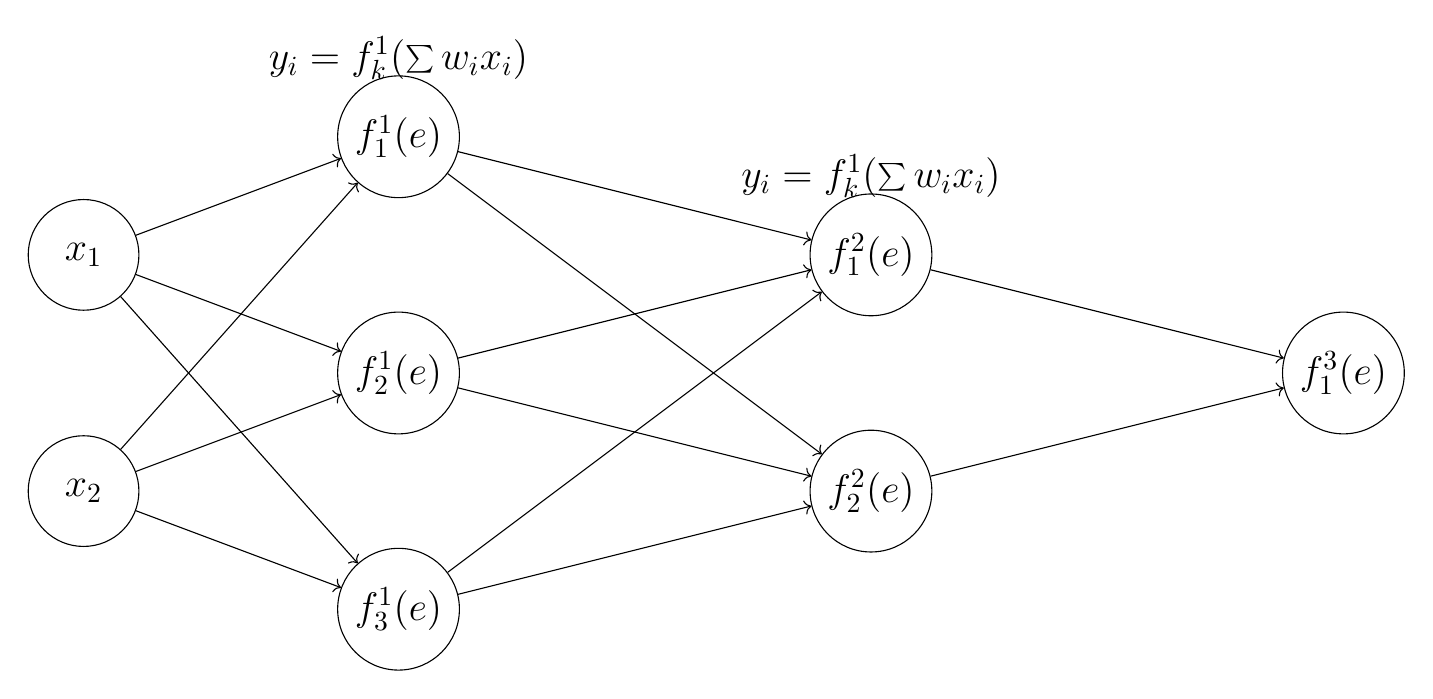
\begin{tikzpicture}
\tikzstyle{neuron}=[circle,draw, minimum size=4em, font=\Large]
\tikzstyle{update}=[dashed, blue]

\coordinate (x_1) at (-5, 1.5);
\coordinate (x_2) at (-5, -1.5);

\coordinate (n_1_1) at (-1, 3);
\coordinate (n_1_2) at (-1, 0);
\coordinate (n_1_3) at (-1, -3);

\coordinate (n_2_1) at (5, 1.5);
\coordinate (n_2_2) at (5, -1.5);

\coordinate (n_3_1) at (11, 0);


\node[neuron] (x_1) at (x_1) {$x_{1}$};
\node[neuron] (x_2) at (x_2) {$x_{2}$};

\node[neuron] (n_1_1) at (n_1_1) {$f^{1}_{1}(e)$};
\node[neuron] (n_1_2) at (n_1_2) {$f^{1}_{2}(e)$};
\node[neuron] (n_1_3) at (n_1_3) {$f^{1}_{3}(e)$};

\node[neuron] (n_2_1) at (n_2_1) {$f^{2}_{1}(e)$};
\node[neuron] (n_2_2) at (n_2_2) {$f^{2}_{2}(e)$};

\node[neuron] (n_3_1) at (n_3_1) {$f^{3}_{1}(e)$};


\node[above of=n_1_1] {\Large $y_i = f^{1}_{k}(\sum w_i x_i)$};
\node[above of=n_2_1] {\Large $y_i = f^{1}_{k}(\sum w_i x_i)$};
%\node[above of=n_3_1] {\Large $y_i = f^{1}_{k}(\sum w_i x_i)$};

\draw[->] (x_1) -- (n_1_1);
\draw[->] (x_1) -- (n_1_2);
\draw[->] (x_1) -- (n_1_3);
\draw[->] (x_2) -- (n_1_1);
\draw[->] (x_2) -- (n_1_2);
\draw[->] (x_2) -- (n_1_3);

\draw[->] (n_1_1) -- (n_2_1);
\draw[->] (n_1_1) -- (n_2_2);
\draw[->] (n_1_2) -- (n_2_1);
\draw[->] (n_1_2) -- (n_2_2);
\draw[->] (n_1_3) -- (n_2_1);
\draw[->] (n_1_3) -- (n_2_2);

\draw[->] (n_2_1) -- (n_3_1);
\draw[->] (n_2_2) -- (n_3_1);

\end{tikzpicture}
}
    \end{figure}
\end{frame}

\subsection{El desvanecimiento del gradiente}
\begin{frame}{\titulo}{\subtitulo}
	\begin{figure}[H]
        \centering
        %\scalebox{0.6}{% http://staff.itee.uq.edu.au/janetw/cmc/chapters/BackProp/index2.html
% http://outlace.com/Beginner-Tutorial-Backpropagation/
% http://neuralnetworksanddeeplearning.com/chap2.html
% http://staff.itee.uq.edu.au/janetw/cmc/chapters/BackProp/slides/Backprop_files/frame.htm
% http://staff.itee.uq.edu.au/janetw/cmc/chapters/BackProp/
% http://home.agh.edu.pl/~vlsi/AI/backp_t_en/backprop.html
% https://www.google.cl/webhp?sourceid=chrome-instant&ion=1&espv=2&ie=UTF-8#safe=off&q=backpropagation+practice+example
% https://ayearofai.com/rohan-4-the-vanishing-gradient-problem-ec68f76ffb9b#.9ntv81akz

\ifx\du\undefined
  \newlength{\du}
\fi
\newcommand{\nweigth}[2]{$W^{#1}_{#2} - \alpha\frac{\partial J}{\partial W^{#1}_{#2}}$}
\newcommand{\w}[2]{$W^{#1}_{#2}$}

\setlength{\du}{1\unitlength}
\begin{tikzpicture}[font=\small]
\tikzstyle{neuron}=[circle,draw, minimum size=2em]
\tikzstyle{update}=[dashed, blue]

\pgftransformxscale{1.000000}
\pgftransformyscale{-1.000000}

\coordinate (x1)    at (0.000000\du, 0.000000\du);
\coordinate (x2)    at (0.000000\du, 8.000000\du);

\coordinate (i)     at (3.000000\du, 0.000000\du);
\coordinate (ii)    at (3.000000\du, 8.000000\du);

\coordinate (iv)    at (10.000000\du, 0.000000\du);
\coordinate (v)     at (10.000000\du, 8.000000\du);

\coordinate (vii)   at (17.000000\du, 0.000000\du);
\coordinate (viii)  at (17.000000\du, 8.000000\du);

\coordinate (ix)   at (17.000000\du, 0.000000\du);
\coordinate (diez)  at (17.000000\du, 8.000000\du);


\coordinate (x)     at (24.000000\du, 4.000000\du);
\coordinate (y)     at (27.000000\du, 4.000000\du);


%%%%%%%%%%%%%%%%%%%%%%%%%%%%%%%%%%%%%%%%%%%%%%%%%%%%%%%%%%
% ENTRADA
\node (X1) at (x1) {\Huge $x_1$};
\node (X2) at (x2) {\Huge $x_2$};

% CAPA DE ENTRADA
\node[neuron] (A) at  (i) {}; % A
\node[neuron] (B) at  (ii)  {}; % B

% CAPA 1
\node[neuron] (C) at  (iv)  {}; % C
\node[neuron] (D) at  (v)  {}; % D

% CAPA 2
\node[neuron] (E) at  (vii)  {}; % E
\node[neuron] (F) at  (viii)  {}; % F

% CAPA 2
\node[neuron] (H) at  (ix)  {}; % E
\node[neuron] (I) at  (diez)  {}; % F

% CAPA DE SALIDA
\node[neuron] (G) at  (x)  {}; % G

% SALIDA
\node (out) at (y) {\Huge $y_1$};
%%%%%%%%%%%%%%%%%%%%%%%%%%%%%%%%%%%%%%%%%%%%%%%%%%%%%%%%%%


\draw[->] (X1) -- (A);
\draw[->] (X2) -- (B);


%%%%%%%%%%%%%%%%%%%%%%%%%%%%%%%%%%%%%%%%%%%%%%%%%%%%%%%%%%
%%%%%%%%%%%%%%%%%%%%%%%%%%%%%%%%%%%%%%%%%%%%%%%%%%%%%%%%%%
\draw[->] (A) -- node[above, pos=0.2] (W_1_11) {\w{1}{11}} (C);
\draw[->] (A) -- node[left , pos=0.2] (W_1_12) {\w{1}{12}} (D);
\draw[->] (B) -- node[left , pos=0.2] (W_1_13) {\w{1}{13}} (C);
\draw[->] (B) -- node[below, pos=0.2] (W_1_14) {\w{1}{14}} (D);

%\draw[->, dashed, blue] (C) to [bend left=40] node[above] {$W^{1}_{11} - \alpha\frac{\partial J}{\partial W^{1}_{11}}$} (W_1_11);
\draw[->, update] (C) to [bend left=40] node[above] {\nweigth{1}{11}} (W_1_11);
\draw[->, update] (D) to [bend left=50] node[above right, pos=0.98] {\nweigth{1}{12}} (W_1_12);

\draw[->, update] (C) to [bend right=50] node[below right, pos=0.98] {\nweigth{1}{13}} (W_1_13);
\draw[->, update] (D) to [bend right=40] node[below] {\nweigth{1}{14}} (W_1_14);

%%%%%%%%%%%%%%%%%%%%%%%%%%%%%%%%%%%%%%%%%%%%%%%%%%%%%%%%%%
%%%%%%%%%%%%%%%%%%%%%%%%%%%%%%%%%%%%%%%%%%%%%%%%%%%%%%%%%%
\draw[->] (C) -- node[above, pos=0.2] (W_2_11) {\w{l}{11}} (E);
\draw[->] (C) -- node[left , pos=0.2] (W_2_12) {\w{2}{12}} (F);
\draw[->] (D) -- node[left , pos=0.2] (W_2_13) {\w{2}{13}} (E);
\draw[->] (D) -- node[below, pos=0.2] (W_2_14) {\w{2}{14}} (F);

\draw[->, update] (E) to [bend left=40] node[above] {\nweigth{2}{11}} (W_2_11);
\draw[->, update] (F) to [bend left=50] node[above right, pos=0.98] {\nweigth{2}{12}} (W_2_12);

\draw[->, update] (E) to [bend right=50] node[below right, pos=0.98] {\nweigth{2}{13}} (W_2_13);
\draw[->, update] (F) to [bend right=40] node[below] {\nweigth{2}{14}} (W_2_14);

%%%%%%%%%%%%%%%%%%%%%%%%%%%%%%%%%%%%%%%%%%%%%%%%%%%%%%%%%%
%%%%%%%%%%%%%%%%%%%%%%%%%%%%%%%%%%%%%%%%%%%%%%%%%%%%%%%%%%
\draw[->] (E) -- node[right, pos=0.2] (W_3_11) {\w{3}{11}} (G);
\draw[->] (F) -- node[right, pos=0.2] (W_3_12) {\w{3}{12}} (G);

\draw[->, update] (G) to [bend  left=50] node[above right, pos=0.98] {\nweigth{3}{11}} (W_3_11);
\draw[->, update] (G) to [bend right=40] node[below right, pos=0.98] {\nweigth{3}{12}} (W_3_12);


\draw[->] (G) -- (out);
\end{tikzpicture}
}
        \scalebox{0.6}{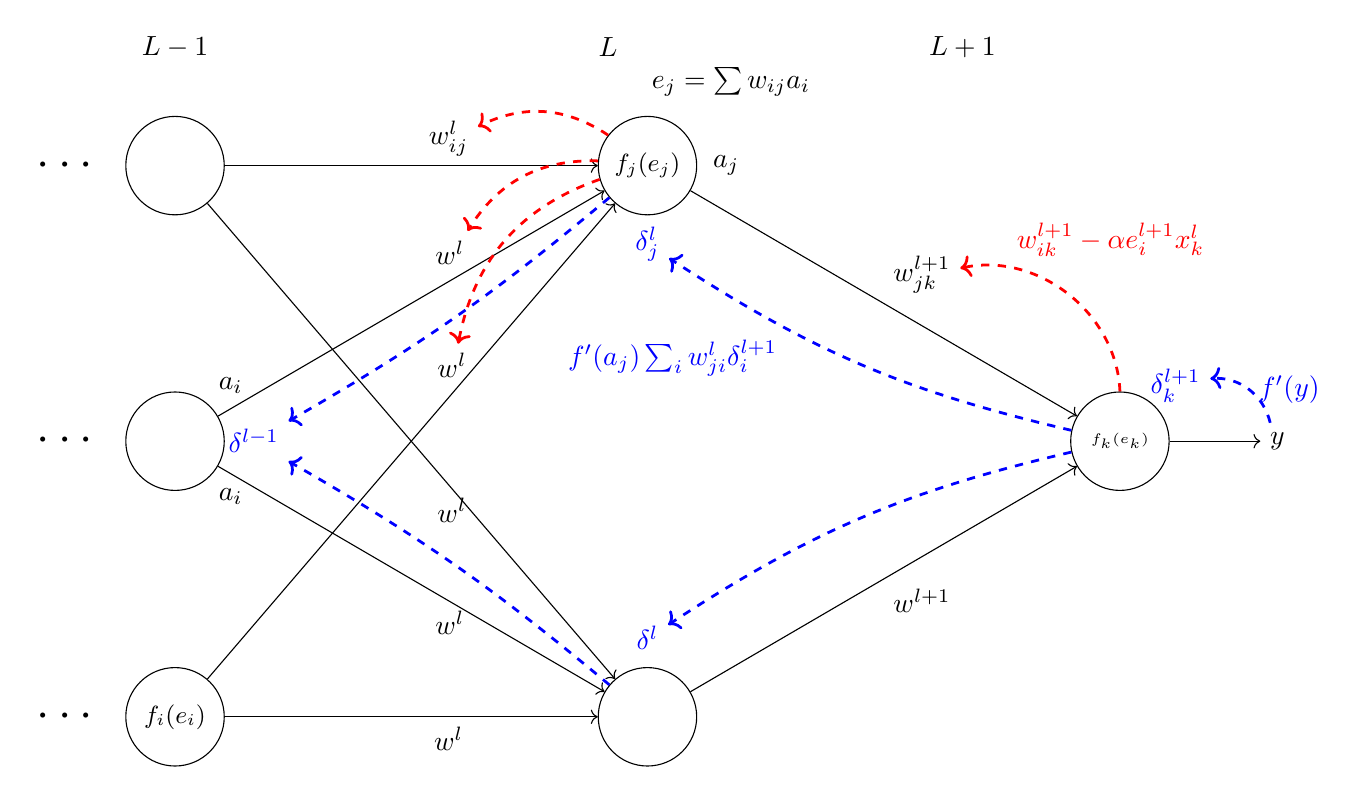
\begin{tikzpicture}

	\tikzstyle{nodo}=[circle, draw, minimum size=1.25cm]
	\tikzstyle{upw}=[dashed, red, ->, line width = 1pt]

	\coordinate (l_0) at (0, 5.0);
	\coordinate (l_1) at (5.5, 5.0);
	\coordinate (l_2) at (10, 5.0);

	\coordinate (f_1_1) at (0, 3.5); % CAPA ENTRADA
	\coordinate (f_1_2) at (0, 0); % CAPA ENTRADA
	\coordinate (f_1_3) at (0, -3.5); % CAPA ENTRADA
	\coordinate (f_2_1) at (6.0, 3.5); % CAPA OCULTA 1
	\coordinate (f_2_2) at (6.0, -3.5); % CAPA OCULTA 1
	\coordinate (f_3_1) at (12, 0); % CAPA SALIDA
	\coordinate (y) at (14, 0); % CAPA SALIDA

	\node[] (l_0) at (l_0) {$L - 1$};
	\node[] (l_1) at (l_1) {$L$};
	\node[] (l_2) at (l_2) {$L + 1$};

	\node[nodo] (f_1_1) at (f_1_1) {}; % CAPA ENTRADA
	\node[nodo] (f_1_2) at (f_1_2) {}; % CAPA ENTRADA
	\node[nodo] (f_1_3) at (f_1_3) {\small $f_i(e_i)$}; % CAPA ENTRADA
	\node[nodo] (f_2_1) at (f_2_1) {\small $f_j(e_j)$}; % CAPA OCULTA 1
	\node[nodo] (f_2_2) at (f_2_2) {}; % CAPA OCULTA 1
	\node[nodo] (f_3_1) at (f_3_1) {\tiny $f_k(e_k)$}; % CAPA SALIDA
	\node[] (y) at (y) {$y$}; % CAPA SALIDA

	\node[left of=f_1_1, node distance=1.4cm] {\LARGE $\cdots$};
	\node[left of=f_1_2, node distance=1.4cm] {\LARGE $\cdots$};
	\node[left of=f_1_3, node distance=1.4cm] {\LARGE $\cdots$};

	\draw[->] (f_1_1) -- node[pos=0.6, above] (w_1_1) {$w^{l}_{ij}$} (f_2_1);
	\draw[->] (f_1_2) -- node[pos=0.6, above] (w_1_2) {$w^{l}_{}$} (f_2_1);
	\draw[->] (f_1_3) -- node[pos=0.6, above] (w_1_3) {$w^{l}_{}$} (f_2_1);
	\draw[->] (f_1_1) node[above right of=f_1_2] {$a_{i}$} -- node[pos=0.6, below] (w_2_1) {$w^{l}_{}$} (f_2_2);
	\draw[->] (f_1_2) node[below right of=f_1_2] {$a_{i}$} -- node[pos=0.6, below] (w_2_2) {$w^{l}_{}$} (f_2_2);
	\draw[->] (f_1_3) -- node[pos=0.6, below] (w_2_3) {$w^{l}_{}$} (f_2_2);
	\draw[->] (f_2_1) node[right of=f_2_1] {$a_{j}$} -- node[pos=0.5, above right] (w_j_k) {$w^{l+1}_{jk}$} (f_3_1);
	\draw[->] (f_2_2) -- node[pos=0.5, below right] {$w^{l+1}$} (f_3_1);
	\draw[->] (f_3_1) -- node[pos=0.5, below right] {$$} (y);

	\node[above right of=f_2_1, node distance=1.5cm] {$e_{j} = \sum w_{ij}a_i$};


	\draw[upw] (f_3_1) to[bend right=50] node[above right, pos=0.8] {$w^{l+1}_{ik} - \alpha e^{l+1}_{i}x^{l}_{k}$} (w_j_k);
	\draw[upw] (f_2_1) to[bend right=30] node[above]{$$} (w_1_1);
	\draw[upw] (f_2_1) to[bend right=30] node[above]{$$} (w_1_2);
	\draw[upw] (f_2_1) to[bend right=30] node[above]{$$} (w_1_3);


	\node[blue, above right of=f_3_1] (e_i) {$\delta^{l+1}_{k}$};
	\node[blue, below of=f_2_1] (e_2_1_i) {$\delta^{l}_{j}$};
	\node[blue, above of=f_2_2] (e_2_2_i) {$\delta^{l}$};
	\node[blue, right of=f_1_2] (e_1_2_i) {$\delta^{l-1}$};

	\draw[upw, blue] (y) to[bend right=40] node[right]{$f'(y)$} (e_i);
	\draw[upw, blue] (f_3_1) to[bend left=10] node[below left, pos=0.7]{$f'(a_{j})\sum_{i}w^{l}_{ji}\delta^{l+1}_{i}$} (e_2_1_i);
	\draw[upw, blue] (f_3_1) to[bend right=10] (e_2_2_i);

	\draw[upw, blue] (f_2_1) to[bend left=5] (e_1_2_i);
	\draw[upw, blue] (f_2_2) to[bend right=5] (e_1_2_i);

\end{tikzpicture}
}
    \end{figure}
\end{frame}



\begin{frame}{\titulo}{\subtitulo}
\maketitle
\end{frame}

%\section{Bibliografía}
%\begin{frame}{\titulo}{\subtitulo}
%    \cite{*}
%    %\cite{Dan}
%    %\cite{Baz}
%    \bibliographystyle{plain}
%    \bibliography{bibliografia}
%\end{frame}
\end{document}
